% Created: 12-FEB-2021
% Revised: 
%
% VERSION 0.1
%
\documentclass{article}

\usepackage{graphicx} % screenshots
\usepackage{fancyhdr} % Required for custom headers
\usepackage{lastpage} % Required to determine the last page for the footer
\usepackage{extramarks} % Required for headers and footers
\usepackage{paralist} % compact lists
\usepackage{parskip} % more space between paragraphs
\usepackage{textcomp} % straight quotes for code
\usepackage{hyperref} % for hyperlinks in the document
\usepackage{tabularx} % for text-wrapping in tables
\usepackage{algorithm} % algorithms
\usepackage{algpseudocode} % algorithms
\usepackage{tikz} % diagrams

% Set up Tikz Library
\usetikzlibrary{shapes.geometric}
\usetikzlibrary{shapes.multipart}
\usetikzlibrary{positioning}
\usetikzlibrary{arrows}
\usetikzlibrary{arrows.meta}
\usetikzlibrary{fit}
\usetikzlibrary{matrix}
\usetikzlibrary{shadows}
\usetikzlibrary{calc}

% Primary key should be underlined
\newcommand{\primarykey}[1]{\underline{#1}}

%%%%% ENTITY %%%%%%

% Entity - Basic rect
\tikzstyle{entity} = [rectangle, draw, thick, black, minimum width=4em, minimum height=2.5em]

% Weak Entity - Double lined rect
\tikzstyle{weak entity} = [entity, double, double distance=2pt]

%%%%% Attribute %%%%%%

% Attribute - Ellipse around attribute
\tikzstyle{attribute} = [ellipse, draw, black, thick, minimum width=5em, minimum height=2em]

% Multi-value attribute - double circled ellipse
\tikzstyle{multi attribute} = [attribute, double, double distance=2pt]

% Derived attribute - Dashed ellipse
\tikzstyle{derived attribute} = [attribute, dashed]

%%%%% Relationship %%%%%%

% Relationship - diamond
\tikzstyle{relationship} = [diamond, draw, black, thick, minimum width=2em, aspect=1, fill=white]

% Weak Entity Relationship - double diamond
\tikzstyle{weak relationship} = [relationship, double, double distance=2pt]

% IS-A relationship - triangle
\tikzstyle{isa} = [isosceles triangle, isosceles triangle apex angle=60, shape border rotate=120, draw, black, thick, minimum size=3em]

%%% Arrow style

\tikzstyle{oneone} = [-{Latex[width=10mm, length=10mm]}, line width=0.2cm]
\tikzstyle{zeroone} = [-{Latex[width=5mm, length=7mm]}]
\tikzstyle{zeromany} = [--]
\tikzstyle{onemany} = [--, line width=0.2cm]


%%% Crow Foot ERD style - PREFIX with ``cf'' %%%


%
% Crow Foot Many
%

\pgfarrowsdeclare{cfmany}{cfmany}
{
  \pgfarrowsleftextend{+-.5\pgflinewidth}%
  \pgfarrowsrightextend{+.5\pgflinewidth}%
}
{
  %\pgfutil@tempdima=0.6pt%
  %\advance\pgfutil@tempdima by.25\pgflinewidth%
  \pgfsetdash{}{+0pt}%
  \pgfsetmiterjoin%
  %\pgfpathmoveto{\pgfqpoint{0pt}{-9\pgfutil@tempdima}}%
  %\pgfpathlineto{\pgfqpoint{-13\pgfutil@tempdima}{0pt}}%
  %\pgfpathlineto{\pgfqpoint{0pt}{9\pgfutil@tempdima}}%
  %\pgfpathmoveto{\pgfqpoint{0\pgfutil@tempdima}{0\pgfutil@tempdima}}%
  \pgfpathmoveto{\pgfqpoint{-15pt}{-6pt}}% 
  \pgfpathlineto{\pgfqpoint{-15pt}{-6pt}}%  
  \pgfpathlineto{\pgfqpoint{-15pt}{6pt}}% 
  \pgfusepathqstroke%
}

%
% Crow Foot zero-Many
%

\pgfarrowsdeclare{cfomany}{cfomany}
{
  \pgfarrowsleftextend{+-.5\pgflinewidth}%
  \pgfarrowsrightextend{+.5\pgflinewidth}%
}
{
  %\pgfutil@tempdima=0.6pt%
  %\advance\pgfutil@tempdima by.25\pgflinewidth%
  \pgfsetdash{}{+0pt}%
  \pgfsetmiterjoin%
  %\pgfpathmoveto{\pgfqpoint{0pt}{-9pt\pgfutil@tempdima}}%
  %\pgfpathlineto{\pgfqpoint{-13pt\pgfutil@tempdima}{0pt}}%
  %\pgfpathlineto{\pgfqpoint{0pt}{9pt\pgfutil@tempdima}}%
  %\pgfpathmoveto{\pgfqpoint{0pt\pgfutil@tempdima}{0pt\pgfutil@tempdima}}%  
  %\pgfpathmoveto{\pgfqpoint{0pt\pgfutil@tempdima}{0pt\pgfutil@tempdima}}%
	\pgfpathmoveto{\pgfqpoint{0pt}{-6pt}}%
  \pgfpathlineto{\pgfqpoint{-13pt}{0pt}}%
  \pgfpathlineto{\pgfqpoint{0pt}{6pt}}%
  %\pgfpathmoveto{\pgfqpoint{0pt\pgfutil@tempdima}{0pt\pgfutil@tempdima}}%  
  %\pgfpathmoveto{\pgfqpoint{0pt\pgfutil@tempdima}{0pt\pgfutil@tempdima}}%
	\pgfpathmoveto{\pgfqpoint{-6pt}{-6pt}}% 
    \pgfpathcircle{\pgfpoint{-16.5pt}{0pt}} {3.5pt}
  \pgfusepathqstroke%
}


%
% Crow Foot One
%

\pgfarrowsdeclare{cfone}{cfone}
{
  \pgfarrowsleftextend{+-.5\pgflinewidth}%
  \pgfarrowsrightextend{+.5\pgflinewidth}%
}
{
  %\pgfutil@tempdima=0.6pt%
  %\advance\pgfutil@tempdima by.25\pgflinewidth%
  \pgfsetdash{}{+0pt}%
  \pgfsetmiterjoin%
  %\pgfpathmoveto{\pgfqpoint{0\pgfutil@tempdima}{0\pgfutil@tempdima}}%
	%\pgfpathmoveto{\pgfqpoint{0.6pt}{0.6pt}}%
  \pgfpathmoveto{\pgfqpoint{-6pt}{-6pt}}% 
  \pgfpathlineto{\pgfqpoint{-6pt}{-6pt}}%  
  \pgfpathlineto{\pgfqpoint{-6pt}{6pt}}% 
  %\pgfpathmoveto{\pgfqpoint{0\pgfutil@tempdima}{0\pgfutil@tempdima}}%
	%\pgfpathmoveto{\pgfqpoint{0.6pt}{0.6pt}}%
  \pgfpathmoveto{\pgfqpoint{-8pt}{-6pt}}% 
  \pgfpathlineto{\pgfqpoint{-8pt}{-6pt}}%  
  \pgfpathlineto{\pgfqpoint{-8pt}{6pt}}%    
  \pgfusepathqstroke%
}

%
% Crow Foot zero-One
%

\pgfarrowsdeclare{cfoone}{cfoone}
{
  \pgfarrowsleftextend{+-.5\pgflinewidth}%
  \pgfarrowsrightextend{+.5\pgflinewidth}%
}
{
  \pgfutil@tempdima=0.6pt%
  %\advance\pgfutil@tempdima by.25\pgflinewidth%
  \pgfsetdash{}{+0pt}%
  \pgfsetmiterjoin%
  %\pgfpathmoveto{\pgfqpoint{0\pgfutil@tempdima}{0\pgfutil@tempdima}}%
  \pgfpathmoveto{\pgfqpoint{-6pt}{-6pt}}% 
  \pgfpathlineto{\pgfqpoint{-6pt}{-6pt}}%  
  \pgfpathlineto{\pgfqpoint{-6pt}{6pt}}% 
  %\pgfpathmoveto{\pgfqpoint{0\pgfutil@tempdima}{0\pgfutil@tempdima}}%
    \pgfpathcircle{\pgfpoint{-12.5pt}{0}} {3.5pt}
  \pgfusepathqstroke%
}

\tikzset{
    zig zag to/.style={
        to path={(\tikztostart) -| ($(\tikztostart)!#1!(\tikztotarget)$) |- (\tikztotarget)}
    },
    zig zag to/.default=0.5,
    cfone to cfone/.style={
        cfone-cfone, zig zag to
    },    
    cfone to cfmany/.style={
        cfone-cfmany, zig zag to,
    },
    cfone to cfomany/.style={
        cfone-cfomany, zig zag to
    },      
    cfmany to cfone/.style={
        cfmany-cfone, zig zag to
    },
    cfmany to cfmany/.style={
        cfmany-cfmany, zig zag to
    },
    cfonemany/.style={
        cfmany-, zig zag to
    },
    cf0many/.style={
        cfomany-, zig zag to
    },
    cfoneone/.style={
        cfone-, zig zag to
    },
    cf0one/.style={
        cfoone-, zig zag to
    }
}
\def\property#1{\node[name=\entityname-#1, every property/.try]{#1};}
\def\properties{\begingroup\catcode`\_=11\relax\processproperties}
\def\processproperties#1{\endgroup%
    \def\propertycode{}%
    \foreach \p in {#1}{%
        \expandafter\expandafter\expandafter\gdef\expandafter\expandafter\expandafter\propertycode%
            \expandafter\expandafter\expandafter{\expandafter\propertycode\expandafter\property\expandafter{\p}\\}%
    }%
    \propertycode%
}

\tikzset{%
    pics/entity/.style n args={3}{code={%
        \node[draw,
        rectangle split,
        rectangle split parts=2,
        text height=1.5ex,
        ] (#1)
        {#2 \nodepart{second}
            \begin{tabular}{>{\raggedright\arraybackslash}p{6em}}
                #3
            \end{tabular}
        };%
    }}
}

\hypersetup{
    colorlinks=true
}

% Set up the header and footer
\pagestyle{fancy}
\lhead{\hmwkAuthorName} % Top left header
\chead{\hmwkTitle} % Top center head
\rhead{\hmwkClass} % Top right header
\lfoot{\lastxmark} % Bottom left footer
\cfoot{} % Bottom center footer
\rfoot{Page\ \thepage\ of\ \protect\pageref{LastPage}} % Bottom right footer
\renewcommand\headrulewidth{0.4pt} % Size of the header rule
%\renewcommand\footrulewidth{0.4pt} % Size of the footer rule

\setlength\parindent{0pt} % Removes all indentation from paragraphs

%----------------------------------------------------------------------------------------
%	DOCUMENT STRUCTURE COMMANDS
%	Skip this unless you know what you're doing
%----------------------------------------------------------------------------------------

% Header and footer for when a page split occurs within a problem environment
\newcommand{\enterProblemHeader}[1]{
% \nobreak\extramarks{#1}{#1 continued on next page\ldots}\nobreak
% \nobreak\extramarks{}{#1 continued on next page\ldots}\nobreak
}

% Header and footer for when a page split occurs between problem environments
\newcommand{\exitProblemHeader}[1]{
% \nobreak\extramarks{#1 (continued)}{#1 continued on next page\ldots}\nobreak
\nobreak\extramarks{#1}{}\nobreak
}

\setcounter{secnumdepth}{0} % Removes default section numbers
\newcounter{homeworkProblemCounter} % Creates a counter to keep track of the number of problems

\newcommand{\homeworkProblemName}{}
\newenvironment{homeworkProblem}[1][Problem \arabic{homeworkProblemCounter}]{ % Makes a new environment called homeworkProblem which takes 1 argument (custom name) but the default is "Problem #"
\stepcounter{homeworkProblemCounter} % Increase counter for number of problems
\renewcommand{\homeworkProblemName}{#1} % Assign \homeworkProblemName the name of the problem
\section{\homeworkProblemName} % Make a section in the document with the custom problem count
\enterProblemHeader{\homeworkProblemName} % Header and footer within the environment
}{
\exitProblemHeader{\homeworkProblemName} % Header and footer after the environment
}

\newcommand{\problemAnswer}[1]{ % Defines the problem answer command with the content as the only argument
\noindent\framebox[\columnwidth][c]{\begin{minipage}{0.98\columnwidth}#1\end{minipage}} % Makes the box around the problem answer and puts the content inside
}

\newcommand{\homeworkSectionName}{}
\newenvironment{homeworkSection}[1]{ % New environment for sections within homework problems, takes 1 argument - the name of the section
\renewcommand{\homeworkSectionName}{#1} % Assign \homeworkSectionName to the name of the section from the environment argument
\subsection{\homeworkSectionName} % Make a subsection with the custom name of the subsection
\enterProblemHeader{\homeworkProblemName\ [\homeworkSectionName]} % Header and footer within the environment
}{
\enterProblemHeader{\homeworkProblemName} % Header and footer after the environment
}

%----------------------------------------------------------------------------------------
%	NAME AND CLASS SECTION
%----------------------------------------------------------------------------------------

\newcommand{\hmwkTitle}{Welcome to K Division} % Assignment title
\newcommand{\hmwkDueDate}{March 8, 2021} % Due date
\newcommand{\hmwkClass}{CP490} % Course/class
\newcommand{\hmwkClassTime}{TBD} % Class/lecture time
\newcommand{\hmwkClassInstructor}{TBD} % Teacher/lecturer
\newcommand{\hmwkAuthorName}{Mr. Klein} % Your name

%----------------------------------------------------------------------------------------
%	TITLE PAGE
%----------------------------------------------------------------------------------------

\title{
\vspace{2in}
\textmd{\textbf{\hmwkClass:\ \hmwkTitle}}\\
\normalsize\vspace{0.1in}\hmwkDueDate\\
\vspace{0.1in}\large{\textit{\hmwkClassInstructor\ \hmwkClassTime}}
\vspace{3in}
}

\author{\textbf{\hmwkAuthorName}}
\date{} % Insert date here if you want it to appear below your name

\begin{document}

\maketitle\thispagestyle{empty}

%----------------------------------------------------------------------------------------
%	Course Parameters
%----------------------------------------------------------------------------------------
\begin{homeworkProblem}[Overview]

  You are going to be part of a fictional, global corporation that produces interactive cloud applications. You will be split into teams. Each team will own a specific part of the application and you will be responsible for designing, programming, and deploying it. You will need to interact with your peer teams to ensure that all parts of the application work together. You will also need to interact with the product owner to ensure that your deliverables meet requirements, and interact with a fictional operations team who will also stand up your application.

\begin{homeworkSection}{Course Format}
  The class will meet as a whole 3 times per week for an hour. During that meeting, time will be spent on:
	\begin{compactitem}
		\item (15 minutes) Team status (3 x 5 minutes)
		\item (30 minutes) Architecture / Design / Document Reviews, as needed
		\item (30 minutes) Problem solving or bootstrapping
	\end{compactitem}

	Team status is a summary of activities -- what your team worked on, and what's up next.
	
	Teams will need to present their solutions to the group for feedback and review. Teams should be prepared to discuss the technical details of the problems they are solving. Teams should be prepared with any diagrams and supporting reference material so that the class is able to understand and contribute feedback. Discussion is to be focussed on gaps and potential trouble areas.

	The time can also be used to help teams solve problems encountered, whether that's a technical issue or help in coordinating deliverables between teams.
	
	Lastly, this project is likely to use technology unfamiliar to the class. I will lead sessions to cover this material.
\end{homeworkSection}


\begin{homeworkSection}{Evaluation Criteria}
	This class is PASS / FAIL, so no graded marks are given. A PASS in this class is earned by demonstrating that you provided value to your team and helped achieve its goals. Failure would represent individuals that did not contribute technically, were unable to work within agreed-upon processes, and could not coordinate with other teams.
	
	You will write a summary of your individual contributions to the project to help with this, which I will combine with my own observations.
\end{homeworkSection}


\begin{homeworkSection}{General Expectations}
	I am going to hold you to the same standards that I have for junior development staff. That is, I know you're capable of doing the work, and you will need help learning the tools and processes.

	While I hope that the class as a whole produces a working application that everyone can take pride in, it's entirely possible that it won't come together as expected. That's ok -- my goal is that you work within software processes, talk with other teams, debate your ideas, and learn unfamiliar tools.

	To that end, we will operate according to these values:

	\begin{compactitem}
		\item \textbf{Respect always}: Assume that people are acting in good faith. Earn the trust of your teammates and give it, too.
		\item \textbf{Fundamentals first}: Value the basics of testing, designing, and communicating. Creating complex solutions is possible through the diligent, regular application of focussed effort. Know your tools and practice.
		\item \textbf{Start simple and iterate}: Value taking action above waiting for answers. Reach out instead of disengaging. Sharing a partial solution today is far more valuable than trying to have everything working next week.
	\end{compactitem}
\end{homeworkSection}

\end{homeworkProblem}


%----------------------------------------------------------------------------------------
%	Problem description
%----------------------------------------------------------------------------------------
\begin{homeworkProblem}[Project]

  K Division produces a platform for multiplayer online text-based roleplaying games\footnote{that is, MUDs: \url{https://en.wikipedia.org/wiki/MUD}} using their proprietary, leading--edge COAL Engine\footnote{\textbf{C}oncurrent \textbf{O}nline \textbf{A}dventure \textbf{L}and Engine}. Since they're a startup, the game engine isn't written yet, so some of you are going to need to do that. They don't have a front-end yet, either. Or a database backend. It's not much of a company, really, but the investors are thrilled!


\begin{homeworkSection}{Background}
	MUDs, and their single--player cousins, the Text Adventure, were precursors to Massively Multiplayer Online Roleplaying Games (MMORPGs). Players connect to a server using a command line terminal, read descriptions of the environment their characters are in, and type commands. Those commands allow the player to travel, engage in combat, manage inventory, craft, and interact with other players.
	
	If you haven't played one of these, then you might want to try \href{https://play.achaea.com/}{Achaea}, which is a rather more sophisticated version of what we're trying to create.

	Why text-based? If it's going to be a \textit{game}, why not have it be in Unity or Unreal? From a systems design standpoint, that would place emphasis in the wrong place. Rather, formulating the project this way provides a frame for a multi--tier application with a user interface, database, and API, along with integration with other software platforms. Insofar as this is a \textit{game}, it's a rather serious one.
\end{homeworkSection}

\begin{homeworkSection}{Playing the Game}
	In the game, a user takes on the role of a character that wanders around a virtual world, solving puzzles, battling monsters and other characters, amassing various items, and conversing with other users.
	
	The user is presented with a text description of their character's current location and a command line prompt. For example\footnote{This is from \textit{Zork I: The Great Underground Empire} (Infocom, 1980)},

	\begin{verbatim}
		West of House
		You are standing in an open field west
		of a white house, with a boarded front
		door.
		There is a small mailbox here.

		>
	\end{verbatim}

	You can see the various parts of text:
	\begin{compactitem}
		\item \textbf{title}: West of House
		\item \textbf{description}: You are standing in \dots
		\item \textbf{item list}: A small mailbox
		\item \textbf{prompt}: The `$>$' character
	\end{compactitem}

	Descriptions may also include lists of:

	\begin{compactitem}
		\item valid exits, insofar as the player character can see
		\item other player characters in the same place
		\item monsters (non--player characters)
	\end{compactitem}
	
	The user then types a command. For example, \texttt{GO EAST} or \texttt{OPEN MAILBOX}.
	
	The game processes the command and replies with a new description, and another prompt. That's it -- that is the core interface and gameplay. That is,

	\begin{compactitem}
		\item The game server presents a block of text
		\item User types in a command
		\item Game server processes text, updating the game state
		\item Repeat!
	\end{compactitem}
\end{homeworkSection}


\begin{homeworkSection}{Game Objects}
	There are four types of objects in the COAL engine:
	\begin{compactitem}
		\item \textbf{Rooms}: These are the locations inhabited by the player characters
		\item \textbf{Items}: Objects that the player character interact with, such as boxes, lanterns, weapons, etc.
		\item \textbf{Characters}: The internal representation of a user's character, capturing the game state
		\item \textbf{Events}: These define how the game engine responds to user commands
	\end{compactitem}

\begin{table}
	\begin{tabularx}{\textwidth}{|r|X|}
		\hline
		Property & Description \\
		\hline \hline
		Title & Short name for a room, e.g. \texttt{West of House} \\
		Description & Longer text with details of what the room looks like \\
		Exits & A list of visible directions mapped to destinations, e.g. \texttt{East $\rightarrow$ House} \\
		\hline
	\end{tabularx}
	\caption{Room properties}
	\label{tab:room-properties}
\end{table}

\begin{table}
	\begin{tabularx}{\textwidth}{|r|X|}
		\hline
		Property & Description \\
		\hline \hline
		Name & Short name for the item, e.g. \texttt{Sting} \\
		Aliases & Other words that can be used for the item, e.g. \texttt{sword} \\
		Description & Additional details, e.g. \texttt{An Elvish short-sword that is somewhat fond of spiders} \\
		Properties & A dictionary of key--value pairs for metadata (like attack value) \\
		Location & Current room the object is in (or none, if it's inside something else or in a player's inventory) \\
		\hline
	\end{tabularx}
	\caption{Item properties}
	\label{tab:item-properties}
\end{table}

\begin{table}
	\begin{tabularx}{\textwidth}{|r|X|}
		\hline
		Property & Description \\
		\hline \hline
		Name & In--game name of the player character \\
		Player & User account the character belongs to \\
		Location & Room where the character is located \\
		Inventory & Items acquired by the player character \\
		Properties & A dictionary of key--value pairs for keeping game state (e.g. \texttt{HAS-SEEN-WELCOME-TEXT} $\rightarrow$ \texttt{TRUE}) \\
		\hline
	\end{tabularx}
	\caption{Character properties}
	\label{tab:character-properties}
\end{table}

\begin{table}
	\begin{tabularx}{\textwidth}{|r|X|}
		\hline
		Property & Description \\
		\hline \hline
		Command & Static text with (optionally) variables describing the syntax of the action, e.g. \texttt{GIVE !ITEM TO !CHARACTER}. This can be an empty string, which is seen as an Event run every turn. \\
		Conditions & A list of Event Items, where all the conditions of given event must be met for the True actions to execute. Otherwise, the False actions will be run. If there are no conditions, the True actions are run. \\
		True actions & A list of Event Items that manipulates the game state if all of the event conditions are all met, or if there are no event conditions. \\
		False actions & A list of Event Items that manipulates the game state if any of the event conditions are not met. \\
		\hline
	\end{tabularx}
	\caption{Event properties}
	\label{tab:event-properties}
\end{table}

\begin{table}
	\begin{tabularx}{\textwidth}{|r|X|}
		\hline
		Property & Description \\
		\hline \hline
		Primitive & A game engine function. For example, to display a message to the user, the game engine function is \texttt{display\_message}. \\
		Arguments & Arguments to the game engine function. For example, \textit{which} message to display. \\
		\hline
	\end{tabularx}
	\caption{Event item properties}
	\label{tab:event-item-properties}
\end{table}

	Each of the object types has a number of \textit{properties}. Those properties are either \textit{mutable}, meaning that they can be changed as part of playing the game, or \textit{immutable}. Properties that are immutable can only be edited by game authors outside of the game and cannot be changed through player interactions directly.

	The locations in the game are collectively referred to as ``rooms,'' even though they could be describing outdoor locations, caves, spaceships, or more abstract settings\footnote{For example, \href{https://en.wikipedia.org/wiki/A_Mind_Forever_Voyaging}{A Mind Forever Voyaging} (Infocom, 1985)}. A list of properties is given in Table \ref{tab:room-properties}. When a user enters a room, the full description is shown. A list of directions, like \texttt{NORTH} or \texttt{UP} are mapped against other rooms, connecting them. This list of exits is usable by, and shown to, the player. The title, description, and exits are all immutable properties.

	Items are what users manipulate in the game: weapons, armour, keys, treasure, and so on. The properties of items are given in Table \ref{tab:item-properties}. An item has a name, but also possibly aliases. For example, there may be a book with the name \textit{Hitchhiker's Guide} that also has an alias of \textit{book} and \textit{guide}, so the user can type: \texttt{GET HITCHHIKER'S GUIDE} or \texttt{GET GUIDE} or \texttt{GET BOOK} interchangeably. Items may have other attributes, too. For example, if the game has combat elements, then items could have attack or defense values. Last, the only mutable property is the item location, since items (in general) can be added to a player character or monster inventory.

	Table \ref{tab:character-properties} lists the properties of player characters. These are the proxies for users, and so all the state in this object is mutable. Additional properties allow the game engine to track game state. For example, the player character may be poisoned, or under the influence of a potion that lasts for a given number of moves. This key--value mechanism provides an open--ended way to create and manage character data. Each character is associated with one and only one player account, but a player account may have multiple player characters.

	Last, the properties of events are given in Table \ref{tab:event-properties}. The functionality of the game is described using events. All the properties are immutable. The game engine considers each event command string as a pattern -- it will try to match the user input against a single action. Once the engine has has determined which event to execute, all of the conditions for that action are evaluated. If they are all met (or if there are no conditions), then the true actions are evaluated. Otherwise, the false actions are evaluated. The true or false actions dictate actual changes to the state of the game -- moving characters from room to room, manipulating items, and any other game mechanics. The conditions and actions have the same format, given in Table \ref{tab:event-item-properties}. A \textit{primitive} is an actual function in the game engine. Content creators will need to have a list of these functions in order to author the game. The arguments given to the primitives are strings, but can be constants or variable names that are part of the command definition.
\end{homeworkSection}

\begin{homeworkSection}{Creating Game Content}
	Game play requires game content. Classically, in MUDs, once you attained a certain rank within the game\footnote{sometimes called wizard status}, you were allowed to author game content. For some early or small MUDs, this meant recompiling the source code. The prevailing idea, however, was that you could add new content as meta--commands in the game.

	For this project, game content creation is separate from game play, but an integral part of the platform. Users should be able to create rooms, items, monsters, and events. The API is designed with the idea that all game content can be authored in the system. What is exposed from the system is a list of \textit{capabilities} corresponding to the \textit{primitives} discussed in the previous section. Someone designing a MUD should be able to take the exposed functionality and author a complete game. Does the game have a PvP element? It should be programmable enough to allow that. What if there is no combat at all? Or an economy of some sort? It should be possible with the exposed primitives. This places pressure to define a robust set of primitives. I have some ideas, and teams have an opportunity to debate this, but emphasis in the project should be to get the platform working as a whole and not spend excessive time on this until the system is operational as a whole.
	
	What is \textit{missing} from this specification is controlling access to the content creation resources. Teams may want to consider implementing some sort of rudimentary access control as an extension to this specification.
\end{homeworkSection}

\begin{homeworkSection}{Design and Architecture Principles}
  Cloud computing is a popular way of deploying large-scale enterprise business applications. Companies large and small outsource their infrastructure and host their applications with cloud computing companies -- be it Amazon, Microsoft, Google, or others. One reason for Amazon's success as a cloud provider is their emphasis on creating \textit{platforms}. The same website that let them sell books became the same one that lets everyone else sell, well, everything. It's a \textit{platform} for online sales. Further, Amazon Web Services (AWS) is consumed by Amazon internally, meaning that the services Amazon sells are the same ones it uses to run their business.
  
  Similarly, the K Division application is a \textit{platform} for MUDs. The game that we should be able to play at the end of this is a \textit{demonstration of the platform} more than a shrink--wrap product\footnote{read more about this here: \url{https://gist.github.com/chitchcock/1281611}}.
  
  The way we build platforms is through \textit{Application Programming Interfaces} (APIs). APIs are everywhere. Google has \href{https://developers.google.com/apis-explorer}{all kinds}. Zoom? They \href{https://marketplace.zoom.us/docs/api-reference/zoom-api}{have an API}. Do you use Slack? They \href{https://api.slack.com/}{have an API} to write bots. So \href{https://developers.facebook.com/}{does Facebook}. Maybe you play games and use Discord. Here's \href{https://discord.com/developers/docs/intro}{their API}.
  
	An \textit{API} is a kind of programming contract. If I provide your service with input that conforms to your specification, then your service agrees to return a result in a given format. For example, an API can be written to accepts and return JavaScript Object Notation (JSON)\footnote{see \href{https://en.wikipedia.org/wiki/JSON}{Wikipedia}} objects. To describe APIs, we are going to use \href{https://swagger.io/specification/}{OpenAPI documents}. OpenAPI is a way of writing descriptions of API contracts in a way that lets us use other code generation software tools to create clients and servers for us.

  You will be given an OpenAPI document that specifies the public--facing API of the COAL Engine. You will negotiate internal APIs with your peer teams. I expect to be able to write my own game client against this public API and use it to explore your work. You may need to negotiate changes to the public API, if it doesn't let you fulfill your requirements.
\end{homeworkSection}

\begin{homeworkSection}{Application Architecture}
	
\begin{figure}
\centering
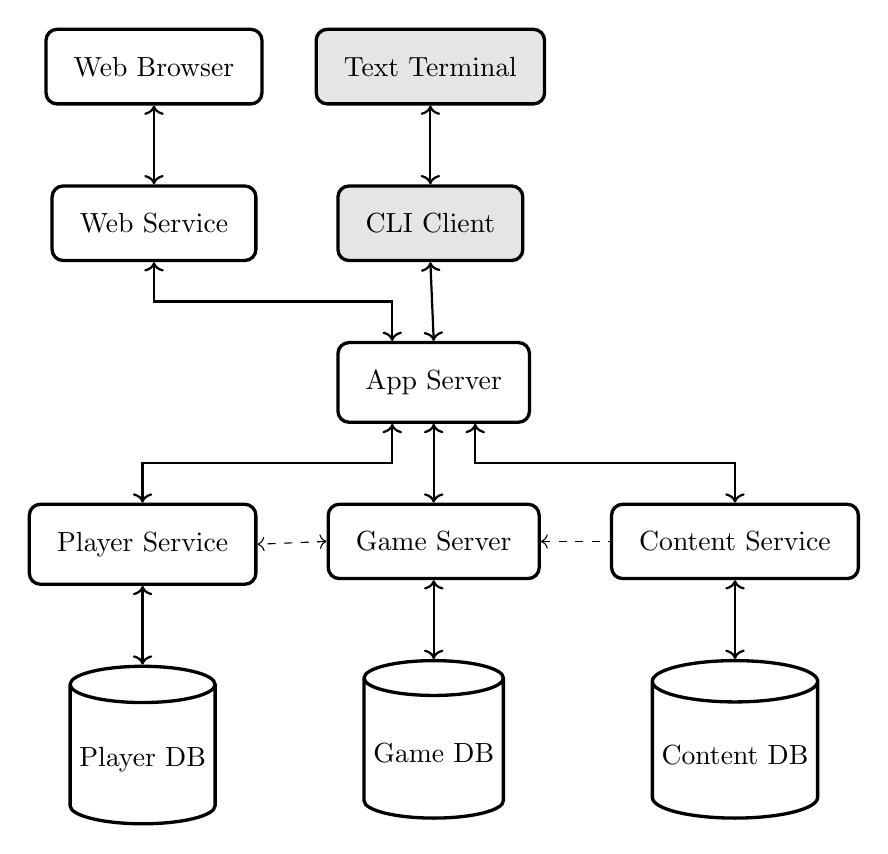
\begin{tikzpicture}
	\tikzset{
    mynode/.style={rectangle,rounded corners, draw=black, very thick, inner sep=1em, text centered},
		usernode/.style={rectangle,rounded corners, draw=black, very thick, inner sep=1em, text centered, fill=black!10},
		dbnode/.style={cylinder,shape border rotate=90,draw=black, very thick, minimum height=2cm, aspect=0.25},
	}
	\node[mynode] (api) at (0,0) {App Server};
	\node[mynode, above left = of api] (webserver) {Web Service};
	\node[mynode, above = of webserver] (webui) {Web Browser};
	\node[usernode, right = of webserver] (cli) {CLI Client};
	\node[usernode, above = of cli] (term) {Text Terminal};

	\draw[<->, thick] (webui.south) -- (webserver.north);

	\draw[<->, thick] (cli.south) --  (api.north);
	\draw[<->, thick] (cli.north) --  (term.south);
	\draw[<->, thick] (webserver.south) -- ++(0, -0.5) -| (api.135);

	\node[mynode, below left = of api] (ps) {Player Service};
	\node[mynode, below = of api] (gs) {Game Server};
	\node[mynode, below right = of api] (cs) {Content Service};

	\draw[<->, thick] (api.225) -- ++(0, -0.5) -| (ps.north);
	\draw[<->, thick] (api.south) -- (gs.north);
	\draw[<->, thick] (api.315) -- ++(0, -0.5) -| (cs.north);

	\draw[<->, dashed] (gs.west) -- (ps.east);
	\draw[<-, dashed] (gs.east) -- (cs.west);

	\node[dbnode, below = of gs] (gdb) {Game DB};
	\node[dbnode, below = of ps] (pdb) {Player DB};
	\node[dbnode, below = of cs] (cdb) {Content DB};

	\draw[<->, thick] (gs.south) -- (gdb.north);
	\draw[<->, thick] (ps.south) -- (pdb.north);
	\draw[<->, thick] (cs.south) -- (cdb.north);
\end{tikzpicture}
\caption{Overall Application Architecture}
\label{fig:arch}
\end{figure}

The overall application architecture is given in Figure \ref{fig:arch}. There are three tiers:
\begin{compactitem}
	\item \textbf{User Interface}: The class is responsible for the web server front--end where users can play the game, manage their account, and so forth.
	\item \textbf{Application Tier}: The application server coordinates activity between the data tier and the UI tiers. It exposes the public API, as given in the OpenAPI specification, and makes corresponding requests to the data tier servers. The server then formats the responses back to the UI clients.
	\item \textbf{Data Tier}: The player, game, and content servers manage their respect portions of the COAL engine. Since each of these services can be expanded in different ways, they each have their own database components. The game service communicates with the player service to update state, as well as the content service to fetch data. 
\end{compactitem}

The class is responsible for all of the components except the \textit{CLI Client}. You will be divided into teams to implement the various servers and database schemas.

Components of the system are described in their own sections below, starting with the REST API itself.
\end{homeworkSection}


\begin{homeworkSection}{Public REST API}
	A REST\footnote{see: \url{https://en.wikipedia.org/wiki/Representational_state_transfer}} API is a way of describing objects and operations against them. A reasonable set of design principles for REST is \href{https://restfulapi.net/}{given here}. In brief, the API has as set of \textit{resources}, or objects in the system, and \textit{methods} used to manipulate them.

	The COAL public API is given in the API Specification PDF. Each URL endpoint is given, along with the expected input parameters, HTTP verb (GET, POST, PUT, or DELETE),  response code (200, 201, etc.) and output format. All data is transferred via JSON documents.

	The \texttt{/game} endpoint corresponds to a particular instance of a MUD. Each instance can be completely different -- different game logic, different game content, and so forth. Having different games is the platform aspect of this application.

	Objects within the game correspond to sub--resources of the \texttt{/game} endpoint:
	\begin{compactitem}
		\item \texttt{/game/\{game\_id\}/room}: Manipulate rooms; see Table \ref{tab:room-properties}
		\item \texttt{/game/\{game\_id\}/item}: Manipulate items; see Table \ref{tab:item-properties}
		\item \texttt{/game/\{game\_id\}/event}: Manipulate events; see Table \ref{tab:event-properties} and Table \ref{tab:event-item-properties}
	\end{compactitem}
	
	Users have accounts with COAL in the form of player objects. Signing up with a server is a call against the \texttt{/player} endpoint. While characters can be retrieved as a sub--resource: \texttt{/player/\{player\_id\}/character}, creating a character is a function of the game server. 
	
	That is, creating a character is a POST to:
	 
	\texttt{/game/\{game\_id\}/player/\{player\_id\}/character} 
	
	The game server is responsible for creating the character and establishing any initial properties for it.
\end{homeworkSection}


\begin{homeworkSection}{Web Service}
	The web service provides the front--end for the game. Users must be able to manage their account and game characters. They must also be able to play the game itself using an interactive console.
\end{homeworkSection}


\begin{homeworkSection}{App Server}
	The App Server is a bridge between the public API and all of the internal components of the application. It has no direct access to the databases, and does not know how the data is stored. Instead, it accepts incoming requests from users and translates them into messages for the internal services and then sends back properly formatted responses.
	
	This design is a pattern for providing \textit{horizontal scaling}. Multiple App Servers can be launched to accommodate user load independently of the other services, since those services may themselves have specific ways to use their resources.

	The app server must send and receive JSON content according COAL public OpenAPI specification. You can use the YAML file in the repository to code generate server, if that helps you.
\end{homeworkSection}

\begin{homeworkSection}{Player Service}

\begin{figure}
	\centering		
  \begin{tikzpicture}
    % Entity 1
		\pic {entity={P}{Players}{%
                id \\
                title \\
            }};

		\pic[below = 1.5cm of P] {entity={C}{Characters}{%
                id \\
								game\_id \\
                title \\
            }};

		\pic[right = 1.25cm of C] {entity={S}{Properties}{%
						id \\
						character\_id \\
						title \\
						value \\
				}};

		\pic[left = 1.25cm of C] {entity={I}{Items}{%
				id \\
				character\_id \\
				item\_id \\
		}};

    % Draw the cardinalities
		\draw[cfoneone] (P.south) -- (C.north);
		\draw[cf0many] (C.north) -- (P.south);

		\draw[cfoneone] (C) -- (S);
		\draw[cf0many] (S) -- (C);

		\draw[cfoneone] (C) -- (I);
		\draw[cf0many] (I) -- (C);
		
  \end{tikzpicture}
\caption{Player server data model}
\label{fig:player-db}
\end{figure}
	
	The Player Service is responsible for user accounts and managing the game characters the user creates. Figure \ref{fig:player-db}, shows a basic data model. Players may have multiple characters. Each character has a set of properties and a set of items. The \texttt{item\_id} and \texttt{game\_id} foreign keys belong to the content and game servers respectively.

	Wherever you see \texttt{title} in a data model field, it is a unique, human--readable, one word \textbf{key}. Think of a \texttt{title} as a hashtag. In contrast, \texttt{description} fields are potentially multi--line text fields with as much text as needed. Properties tables are dictionaries or maps of keys (\texttt{titles}) and values; they're an open--ended mechanism for storing data.
	\end{homeworkSection}

\begin{homeworkSection}{Content Service}

	\begin{figure}
		\centering		
		\begin{tikzpicture}
			% Entity 1
			\pic {entity={I}{Items}{%
									id \\
									title \\
									description \\
									location \\
							}};

			\pic [right = 1.25cm of I] {entity={IA}{ItemAliases}{%
							id \\
							item\_id \\
							title \\
					}};

			\pic [left = 1.25cm of I] {entity={P}{Properties}{%
					id \\
					item\_id \\
					title \\
					value \\
			}};

			\pic[below = of I] {entity={R}{Rooms}{%
									id \\
									game\_id \\
									title \\
									description \\
							}};
	
			\pic[right = 1.25cm of R] {entity={E}{Exits}{%
							id \\
							from\_room\_id \\
							to\_room\_id \\
							direction \\
					}};
	
			% Draw the cardinalities
			\draw[cfoneone] (I) -- (IA);
			\draw[cf0many] (IA) -- (I);

			\draw[cfoneone] (I) -- (P);
			\draw[cf0many] (P) -- (I);

			\draw[cfoneone] (R) -- (E);
			\draw[cf0many] (E) -- (R);
			
		\end{tikzpicture}
	\caption{Content server data model}
	\label{fig:content-db}
	\end{figure}
	
	The Content server contains all of the game assets -- text, descriptions, and properties for rooms and items. Figure \ref{fig:content-db} is a basic data model. Items have can have multiple properties and aliases. An Item \texttt{location} is a \texttt{room\_id}. Rooms can have zero or more exits. The \texttt{Exits} table has two foreign key fields that reference the same table. That is, \texttt{from\_room\_id} and \texttt{to\_room\_id} are both \texttt{room\_id} fields references the \texttt{Rooms} table. 
	
	Implied in this schema is that room exits are not reciprocal. That is, just because a character can go \texttt{UP} into a room doesn't mean the character can go back \texttt{DOWN}.
\end{homeworkSection}

\begin{homeworkSection}{Game Service}
	\begin{figure}
		\centering		
		\begin{tikzpicture}
			% Entity 1
			\pic {entity={G}{Game}{%
									id \\
									title \\
									description \\
							}};

			\pic [right = 1.25cm of G] {entity={P}{Properties}{%
				id \\
				game\_id \\
				title \\
				value \\
			}};

			\draw[cfoneone] (G) -- (P);
			\draw[cf0many] (P) -- (G);

			\pic [below = 1.5 cm of G] {entity={E}{Events}{%
				id \\
				game\_id \\
				command \\
			}};

			\draw[cfoneone] (G) -- (E);
			\draw[cf0many] (E) -- (G);

			\pic[right = 1.25cm of E] {entity={C}{Conditions}{%
				id \\
				event\_id \\
				position \\
				primitive \\
			}};

			\draw[cfoneone] (E) -- (C);
			\draw[cf0many] (C) -- (E);

			\pic[right = 1.25cm of C] {entity={CA}{ConditionArgs}{%
				id \\
				event\_item\_id \\
				position \\
				title \\
			}};

			\draw[cfoneone] (C) -- (CA);
			\draw[cf0many] (CA) -- (C);

			\pic[below = of C] {entity={TP}{TruePart}{%
				id \\
				event\_id \\
				position \\
				primitive \\
			}};

			\draw[cfoneone] (E.300) |- (TP);
			\draw[cf0many] (TP.west) -| (E.300);

			\pic[right = 1.25cm of TP] {entity={TA}{TrueArgs}{%
				id \\
				event\_item\_id \\
				position \\
				title \\
			}};

			\draw[cfoneone] (TP) -- (TA);
			\draw[cf0many] (TA) -- (TP);

		\pic[below = of TP] {entity={FP}{FalsePart}{%
			id \\
			event\_id \\
			position \\
			primitive \\
		}};

		\draw[cfoneone] (E.240) |- (FP);
		\draw[cf0many] (FP.west) -| (E.240);

		\pic[right = 1.25cm of FP] {entity={FA}{FalseArgs}{%
		id \\
		event\_item\_id \\
		position \\
		title \\
		}};

		\draw[cfoneone] (FP) -- (FA);
		\draw[cf0many] (FA) -- (FP);

		\end{tikzpicture}
	\caption{Game server data model}
	\label{fig:game-db}
	\end{figure}

	The Game Service is responsible for managing game play. The service will have to reach out to the content service for room and item descriptions, and it will have to reach out to the player service to fetch and update character data. Figure \ref{fig:game-db} has a basic data model. The game engine parses user input (described in the next section), evaluates events with that input, and returns results back to the user.

	While games themselves have a set of properties, the real complexity is in the engine logic, as captured in the \texttt{Events} table and its children. An event has three parts -- conditions to evaluate, steps to follow if those conditions are met, and steps to follow if they do not. All three of these parts consist of ordered lists, and so have a \texttt{position} field. Also, all three of these parts consist of a game engine function, called a \texttt{primitive}, and arguments to that function captured in the \texttt{*Args} tables.

\end{homeworkSection}

\begin{homeworkSection}{Input Parsing}
	Text adventure games and MUDs have all kinds of ways to understand what the user is trying to do with their characters. Turning user text into actions that the game engine can perform is \textit{parsing} the input.

	The COAL engine uses a specific parsing algorithm that's not as sophisticated as some\footnote{For example, the parser used by the \href{http://www.tads.org/t2doc/doc/parser.htm}{Text Adventure Development System (TADS)}}, but also not as simple as the ones used in the first text adventure games\footnote{Specifically, the first commercially successful ones published by \href{https://en.wikipedia.org/wiki/Scott_Adams_(game_designer)}{Scott Adams} in 1978, which understood only two words, and only the first three letters of each word at that.}.

	To start, consider that each \texttt{Event}, as above, has a \texttt{command}. That \texttt{command} is a pattern consisting of words and variables. For example, all of these could be commands in the same game:

	\begin{compactitem}
		\item \texttt{GIVE !ITEM TO !CHARACTER}
		\item \texttt{GIVE !ITEM TO BEAR}
		\item \texttt{GIVE HONEY TO BEAR}
	\end{compactitem}

	In the first command, there are two variables: \texttt{!ITEM} and \texttt{!CHARACTER}. If the user typed: \texttt{GIVE LANTERN TO WIZARD}, then that would be a valid input. However, if the user typed: \texttt{GIVE FOOD FOR BEAR}, then that wouldn't be understood, because \texttt{FOR} isn't part of any of the command patterns.

	The first part of the algorithm, then, is given in Algorithm \ref{alg:coal-part-1}. This part filters out whether there are any matching events at all. Using the algorithm, and the events above, if the user typed: \texttt{GIVE LANTERN TO BEAR}, then the first two events would match. The first because both variables accept the input, and the second because of the \texttt{BEAR} part. The last rule does not match, because the user typed \texttt{LANTERN} and not \texttt{HONEY}.

	\begin{algorithm}
		\caption{COAL Parser, Part 1}
		\label{alg:coal-part-1}
		\begin{algorithmic}
			\Procedure{FindEvents}{$input$}
				\State $w \gets$ number of words in input
				\State $c \gets$ commands of length $w$
				\For{$i \gets 1,w$}\Comment{Look at each word}
					\State $keepers \gets$ empty list
					\For{$r \gets 1,c$}\Comment{Check each event}
						\If{$w[i] = r[i]$ or $r[i]$ is a variable}
							\State $keeprs \gets$ r
						\EndIf
					\EndFor
					\State $c \gets$ keepers
				\EndFor
				\Return $c$
			\EndProcedure
	\end{algorithmic}
	\end{algorithm}

	If there are no matches on the events, an error is returned. A message like, \texttt{I DO NOT UNDERSTAND} could be displayed.

	If only one event is left, then that event can be evaluated (see the next section for a discussion on processing events).

	What do should happen if multiple rules match? Find the most specific one. That is, find the event with that matches that has the fewest variables. In the example, that is this rule: \texttt{GIVE !ITEM TO BEAR}, since this has one variable, and the other rule has two (\texttt{!ITEM} and \texttt{!CHARACTER}).

	\begin{algorithm}
		\caption{COAL Parser, Part 2}
		\label{alg:coal-part-2}
		\begin{algorithmic}
			\Procedure{ReduceEvents}{$input$, $events$}
				\State $w \gets$ number of words in input
				\For{$i \gets 1,w$}
					\If{length($events$) $= 1$}
						\State \textbf{return} $events[0]$
					\EndIf
					\State $keepers \gets$ empty list
					\For{$r \gets 1,events$}
						\If{$w[i] = r[i]$}
							\State $keepers \gets r$
						\EndIf
					\EndFor
					\If{length($keepers$) $>0$}
						\State $events \gets keepers$
					\EndIf
				\EndFor
				\If{length($events$) $>1$}
					\State \textbf{return} ``Error"\Comment{Input is still ambiguous}
				\EndIf
				\State \textbf{return} $events[0]$
			\EndProcedure
		\end{algorithmic}
	\end{algorithm}

	Algorithm \ref{alg:coal-part-2} filters the events from Part 1. Again, this algorithm searches word by word through the user input. All the rules will match -- but if there's a word that matches \textit{exactly} then that event is kept. At the end of the loop through all of the rules, one of two things is true: (a) there is a set of rules with exact matches, or (b) that particular word is a variable in all the events. If (a) is true, then the set of events to process \textit{becomes} the set of matched rules. Otherwise, the algorithm continues onto the next input word.

	At any time, if only one event remains, then the algorithm stops and returns that event. If, at the end of the algorithm, there are still multiple matches, then this represents a problem with the rules themselves -- an ambiguity has been created. The program shouldn't crash at this point, though, but rather return an error.

	One an event has been found, it is evaluated. This evaluation can change game state and produces an output message for the user. The next section details this process.

\end{homeworkSection}

\begin{homeworkSection}{Game Engine Primitives}
	Once user input is parsed and an event identified, it must be evaluated. Game authors need to have the ability to make the game respond to commands, and the way to do this is to expose an API. This API is explicitly designed to manipulate game state, but not content. That is, the API will let you set properties, but not change room descriptions.

	The API consists of functions in the game engine, and arguments to those functions. Arguments can be constant strings or command variables.

	\begin{table}
		\begin{tabularx}{\textwidth}{|r|l|X|}
			\hline
			Primitive & Arguments & Description \\
			\hline \hline
			is\_property\_eq & key, value & Is the character property \textit{key} equal to \textit{value} \\
			is\_property\_gt & key, value & Is the character property \textit{key} greater than \textit{value} \\
			is\_property\_lt & key, value & Is the character property \textit{key} less than \textit{value} \\
			\hline
		\end{tabularx}
		\caption{Event condition primitives}
		\label{tab:event-condition-primitives}
	\end{table}

	There are two classes of functions -- conditions, and actions. Conditions are used to evaluate the game state. For example, \texttt{is\_property\_eq(key, value)} asks whether character property \texttt{key} has a specific value. Each condition has a boolean result. A list of condition primitives is given in Table \ref{tab-event-condition-primitives}.
	
	\begin{table}
		\begin{tabularx}{\textwidth}{|r|l|X|}
			\hline
			Primitive & Arguments & Description \\
			\hline \hline
			message & key & Send the value of global property \textit{key} to the user \\
			set\_key & key, value & Set character property \textit{key} to \textit{value} \\
			look & none & Send a message with the the title, description, list of exits, and items of the character's current room \\
			\hline
		\end{tabularx}
		\caption{Event action primitives}
		\label{tab:event-action-primitives}
	\end{table}

	An action affects the game state. For example, \texttt{message(key)} sends the value of the game property \texttt{key} back to the user. Some actions are given in Table \ref{tab:event-action-primitives}.

	The first part of evaluating an event is to evaluate all of its conditions. If all of its conditions are true, then the list of actions in the \texttt{true\_part} are run. An event may also have \textit{no} conditions, in which case the true actions are run automatically. Otherwise, if any condition is false, then the \texttt{false\_part} actions are run.

	What can happen, then, is that a user can try to a command, have it recognized by the engine, but still result in nothing happening. That's entirely ok.

	Lastly, there is one set of events that are always evaluated. Events may have a command string that is empty. These are global events that run for every character on every input. An example of this is displaying a welcome message to new characters. A global event is defined that checks to see if the \texttt{first-time} key is set for a character. If it is, then nothing happens (the \texttt{true\_part} is empty). If it isn't set, then: (a) the welcome message is sent, and (b) the \texttt{first-time} key is set.
\end{homeworkSection}


\begin{homeworkSection}{Secondary Objectives}
	There are things missing from this specification. If we get to them, then these would be interesting:
	\begin{compactitem}
		\item \textbf{Engine Primitives}: The lists of actions and conditions is most likely entirely incomplete. I haven't thought enough about authoring a game to work through what a \textit{minimal} set looks like, so I've taken some guesses. If we get to the point of actually getting game content together then it'll make for some good discussion.
		\item \textbf{Access Control}: Content creation is normally reserved for the people running the game server and their designates. The servers should be extended to recognize different user access levels -- player and admin, and restrict all of the content creation endpoints to be admin-only.
		\item \textbf{Non--Player Characters (NPCs)}: A feature of some MUDs are monsters and combat mechanics. Sometimes, there are shop and equipment buying mechanics, too. While this might be possible using item objects, having NPCs as their own content type might be easier.
	\end{compactitem}
\end{homeworkSection}

\end{homeworkProblem}


%----------------------------------------------------------------------------------------
%	Problem description
%----------------------------------------------------------------------------------------
\begin{homeworkProblem}[Tools and Technology]

	\begin{homeworkSection}{Coding Environment}
		It's up to you and your team.
		
		For what it's worth, however, this project was prototyped entirely in Python.
		
		I work on a Microsoft Surface Pro 6 running Windows 10. I use the Windows Subsystem for Linux v2 and run Ubuntu. All of the code and documents were written in \href{https://code.visualstudio.com/}{Visual Studio Code}.
	\end{homeworkSection}

	\begin{homeworkSection}{Hosting}
		Standing up the application and seeing it work over the Internet makes all of this seem more real. Depending on the technology stack your team chooses, there are different places where you can host it for no cost.

		For example, if you want a plain Linux server, then a cloud--based virtual machine (compute instance) would work:
		\begin{compactitem}
			\item Amazon Web Services (\url{https://aws.amazon.com/free}) has a 12 Month Free EC2 compute instance option with 750 hours (roughly a month)
			\item Oracle Cloud (\url{https://www.oracle.com/ca-en/cloud/free}) has an always--free tier with 2 small Linux instances
		\end{compactitem}

		You could use an app hosting service, like Heroku (\url{https://www.heroku.com/pricing}); the free option would also be fine for this course.
	\end{homeworkSection}

	\begin{homeworkSection}{OpenAPI}
		To edit or visualise the COAL specification, use this site: \url{https://editor.swagger.io/}

		The full specification for what OpenAPI is can be found \href{http://spec.openapis.org/oas/v3.0.3}{here}. We are using v3.0.3. A more easily browsable version is \href{https://swagger.io/specification/}{on this site}. Finally, if you want a friendlier explanation of the specification, \href{https://swagger.io/docs/specification/basic-structure/}{go here}.
	\end{homeworkSection}

	\begin{homeworkSection}{Debugging REST}
		One of the challenges in this project will be working with REST servers. Being able to quickly figure out if what you're receiving from the server is correct is going to be important. There are all sorts of tools to help with this -- paid, free, online, offline, \dots

		I like to go with command line tools, and my favourite for this is cURL (\url{https://curl.se/}). It's available for most platforms and can do far more than we'll use here.

		For online options, the \textit{Advanced REST Client} extension for Google Chrome is fairly simple to use. Or maybe \url{https://hoppscotch.io/}.
	\end{homeworkSection}
\end{homeworkProblem}

\end{document}